\documentclass{ximera}

%% You can put user macros here
%% However, you cannot make new environments

\listfiles

\graphicspath{{./}{firstExample/}{secondExample/}}

\usepackage{tikz}
\usepackage{tkz-euclide}
\usepackage{tikz-3dplot}
\usepackage{tikz-cd}
\usetikzlibrary{shapes.geometric}
\usetikzlibrary{arrows}
\usetikzlibrary{decorations.pathmorphing,patterns}
\usetkzobj{all}
\pgfplotsset{compat=1.13} % prevents compile error.

\renewcommand{\vec}[1]{\mathbf{#1}}
\newcommand{\RR}{\mathbb{R}}
\newcommand{\dfn}{\textit}
\newcommand{\dotp}{\cdot}
\newcommand{\id}{\text{id}}
\newcommand\norm[1]{\left\lVert#1\right\rVert}
 
\newtheorem{general}{Generalization}
\newtheorem{initprob}{Exploration Problem}

\tikzstyle geometryDiagrams=[ultra thick,color=blue!50!black]

\usepackage{mathtools}

\title{8.5 Constant Coefficient Equations with Piecewise Continuous Forcing Functions}%\label{Module 7-ADEF}


\begin{document}

\begin{abstract}
We show how Laplace Transforms may be used to solve initial value problems with piecewise continuous forcing functions.
\end{abstract}

\maketitle

\section*{Constant Coefficient Equations with Piecewise Continuous Forcing Functions}

We'll now consider initial value problems of the form
\begin{equation}\label{eq:8.5.1}
 ay''+by'+cy=f(t), \quad  y(0)=k_0,\quad y'(0)=k_1,
\end{equation}
where $a$, $b$, and $c$ are constants ($a\neq 0$) and $f$ is piecewise
continuous on $[0,\infty)$. Problems of this kind occur in situations
where the input to a physical system undergoes instantaneous changes,
as when a switch is turned on or off or the forces acting on the
system change abruptly.

It can be shown %(Exercises~\ref{exer:8.5.23} and \ref{exer:8.5.24}) 
that the differential equation in \eqref{eq:8.5.1} has no solutions on
an open interval that contains a jump discontinuity of $f$. Therefore we
must define what we mean by a solution of \eqref{eq:8.5.1} on $[0,\infty)$
in the case where $f$ has jump discontinuities. The next theorem
motivates our definition. We omit the proof.

\begin{theorem}\label{thmtype:8.5.1}
Suppose $a,b$, and $c$ are constants $(a\neq 0),$ and $f$ is
piecewise  continuous on $[0,\infty).$ with jump discontinuities
at $t_1, \dots, t_n,$ where
$$
0<t_1<\cdots<t_n.
$$
 Let $k_0$ and $k_1$ be arbitrary real numbers. Then there
is a unique function $y$ defined on $[0,\infty)$ with these
properties:
\begin{enumerate}
\item % (a)
 $y(0)=k_0$ and  $y'(0)=k_1$.
\item % (b)
 $y$ and $y'$  are continuous on $[0,\infty)$.
\item % (c)
$y''$ is defined
on every open subinterval of $[0,\infty)$ that does not contain any of the
points $t_1,$ \dots, $t_n$, and
$$
ay''+by'+cy=f(t)
$$
on every such subinterval.
\item % (d)
$y''$ has limits from the right and left at $t_1,$ \dots$,$ $t_n$.
\end{enumerate}
\end{theorem}

We define the function $y$  of Theorem~\ref{thmtype:8.5.1}  to be the
solution of the initial value problem \eqref{eq:8.5.1}.

We begin by considering initial value problems of the form
\begin{equation}\label{eq:8.5.2}
ay''+by'+cy=\left\{\begin{array}{cl} f_0(t),&0\leq
t<t_1,\\f_1(t),&t\geq t_1,
\end{array}\right.\quad y(0)=k_0,\quad y'(0)=k_1,
\end{equation}
where the forcing function has a single jump discontinuity at $t_1$.

We can solve \eqref{eq:8.5.2} by  the these steps:
\begin{procedure}\label{proc:forcingfunctdisc}

\textit{Step 1.} Find the solution $y_0$ of  the initial value problem
$$
ay''+by'+cy=f_0(t), \quad  y(0)=k_0,\quad y'(0)=k_1.
$$
\textit{Step 2.} Compute $c_0=y_0(t_1)$ and $c_1=y_0'(t_1)$.
\textit{Step 3.} Find the solution $y_1$ of  the initial value problem
$$
ay''+by'+cy=f_1(t), \quad  y(t_1)=c_0,\quad y'(t_1)=c_1.
$$
\textit{Step 4.} Obtain the solution $y$ of  \eqref{eq:8.5.2} as
$$
y=\left\{\begin{array}{cl} y_0(t),&0\leq t<t_1\\y_1(t),&t\geq t_1.
\end{array}\right.
$$
\end{procedure}


It 
%is shown  in  Exercise~\ref{exer:8.5.23} 
can be shown that $y'$  exists and is
continuous at $t_1$. The next example illustrates this procedure.

\begin{example}\label{example:8.5.1}
Solve the initial value problem
\begin{equation}\label{eq:8.5.3}
y''+y=f(t),
\quad   y(0)=2,  y'(0)=-1,
\end{equation}
where
$$
f(t)=\left\{\begin{array}{rl}
1,&0\leq t<\frac{\pi}{2},\\
-1,&t\geq \frac{\pi}{2}.
\end{array}\right.
$$
\begin{explanation}
The initial value problem in Step 1 is
$$
y''+y=1, \quad   y(0)=2,\quad y'(0)=-1.
$$
We leave it to you to verify that its solution is
$$
y_0=1+\cos t-\sin t.
$$
Doing Step 2 yields
 $y_0(\pi/2)=0$ and $y_0'(\pi/2)=-1$,
so the second initial value problem is
$$
y''+y=-1, \quad  y\left(\frac{\pi}{2}\right)=0, y'\left(\frac{\pi}{2}\right)=-1.
$$
We leave it to you to verify that the solution of this problem
is
$$
y_1=-1+\cos t+\sin t.
$$
Hence, the solution of \eqref{eq:8.5.3} is
\begin{equation}\label{eq:8.5.4}
y=\left\{\begin{array}{rl}
1+\cos t-\sin t,&0\leq t<\frac{\pi}{2},
\\
-1+\cos t+\sin t,&t\geq \frac{\pi}{2}
\end{array}\right.
\end{equation}
%(Figure:8.5.1).
\begin{image}
 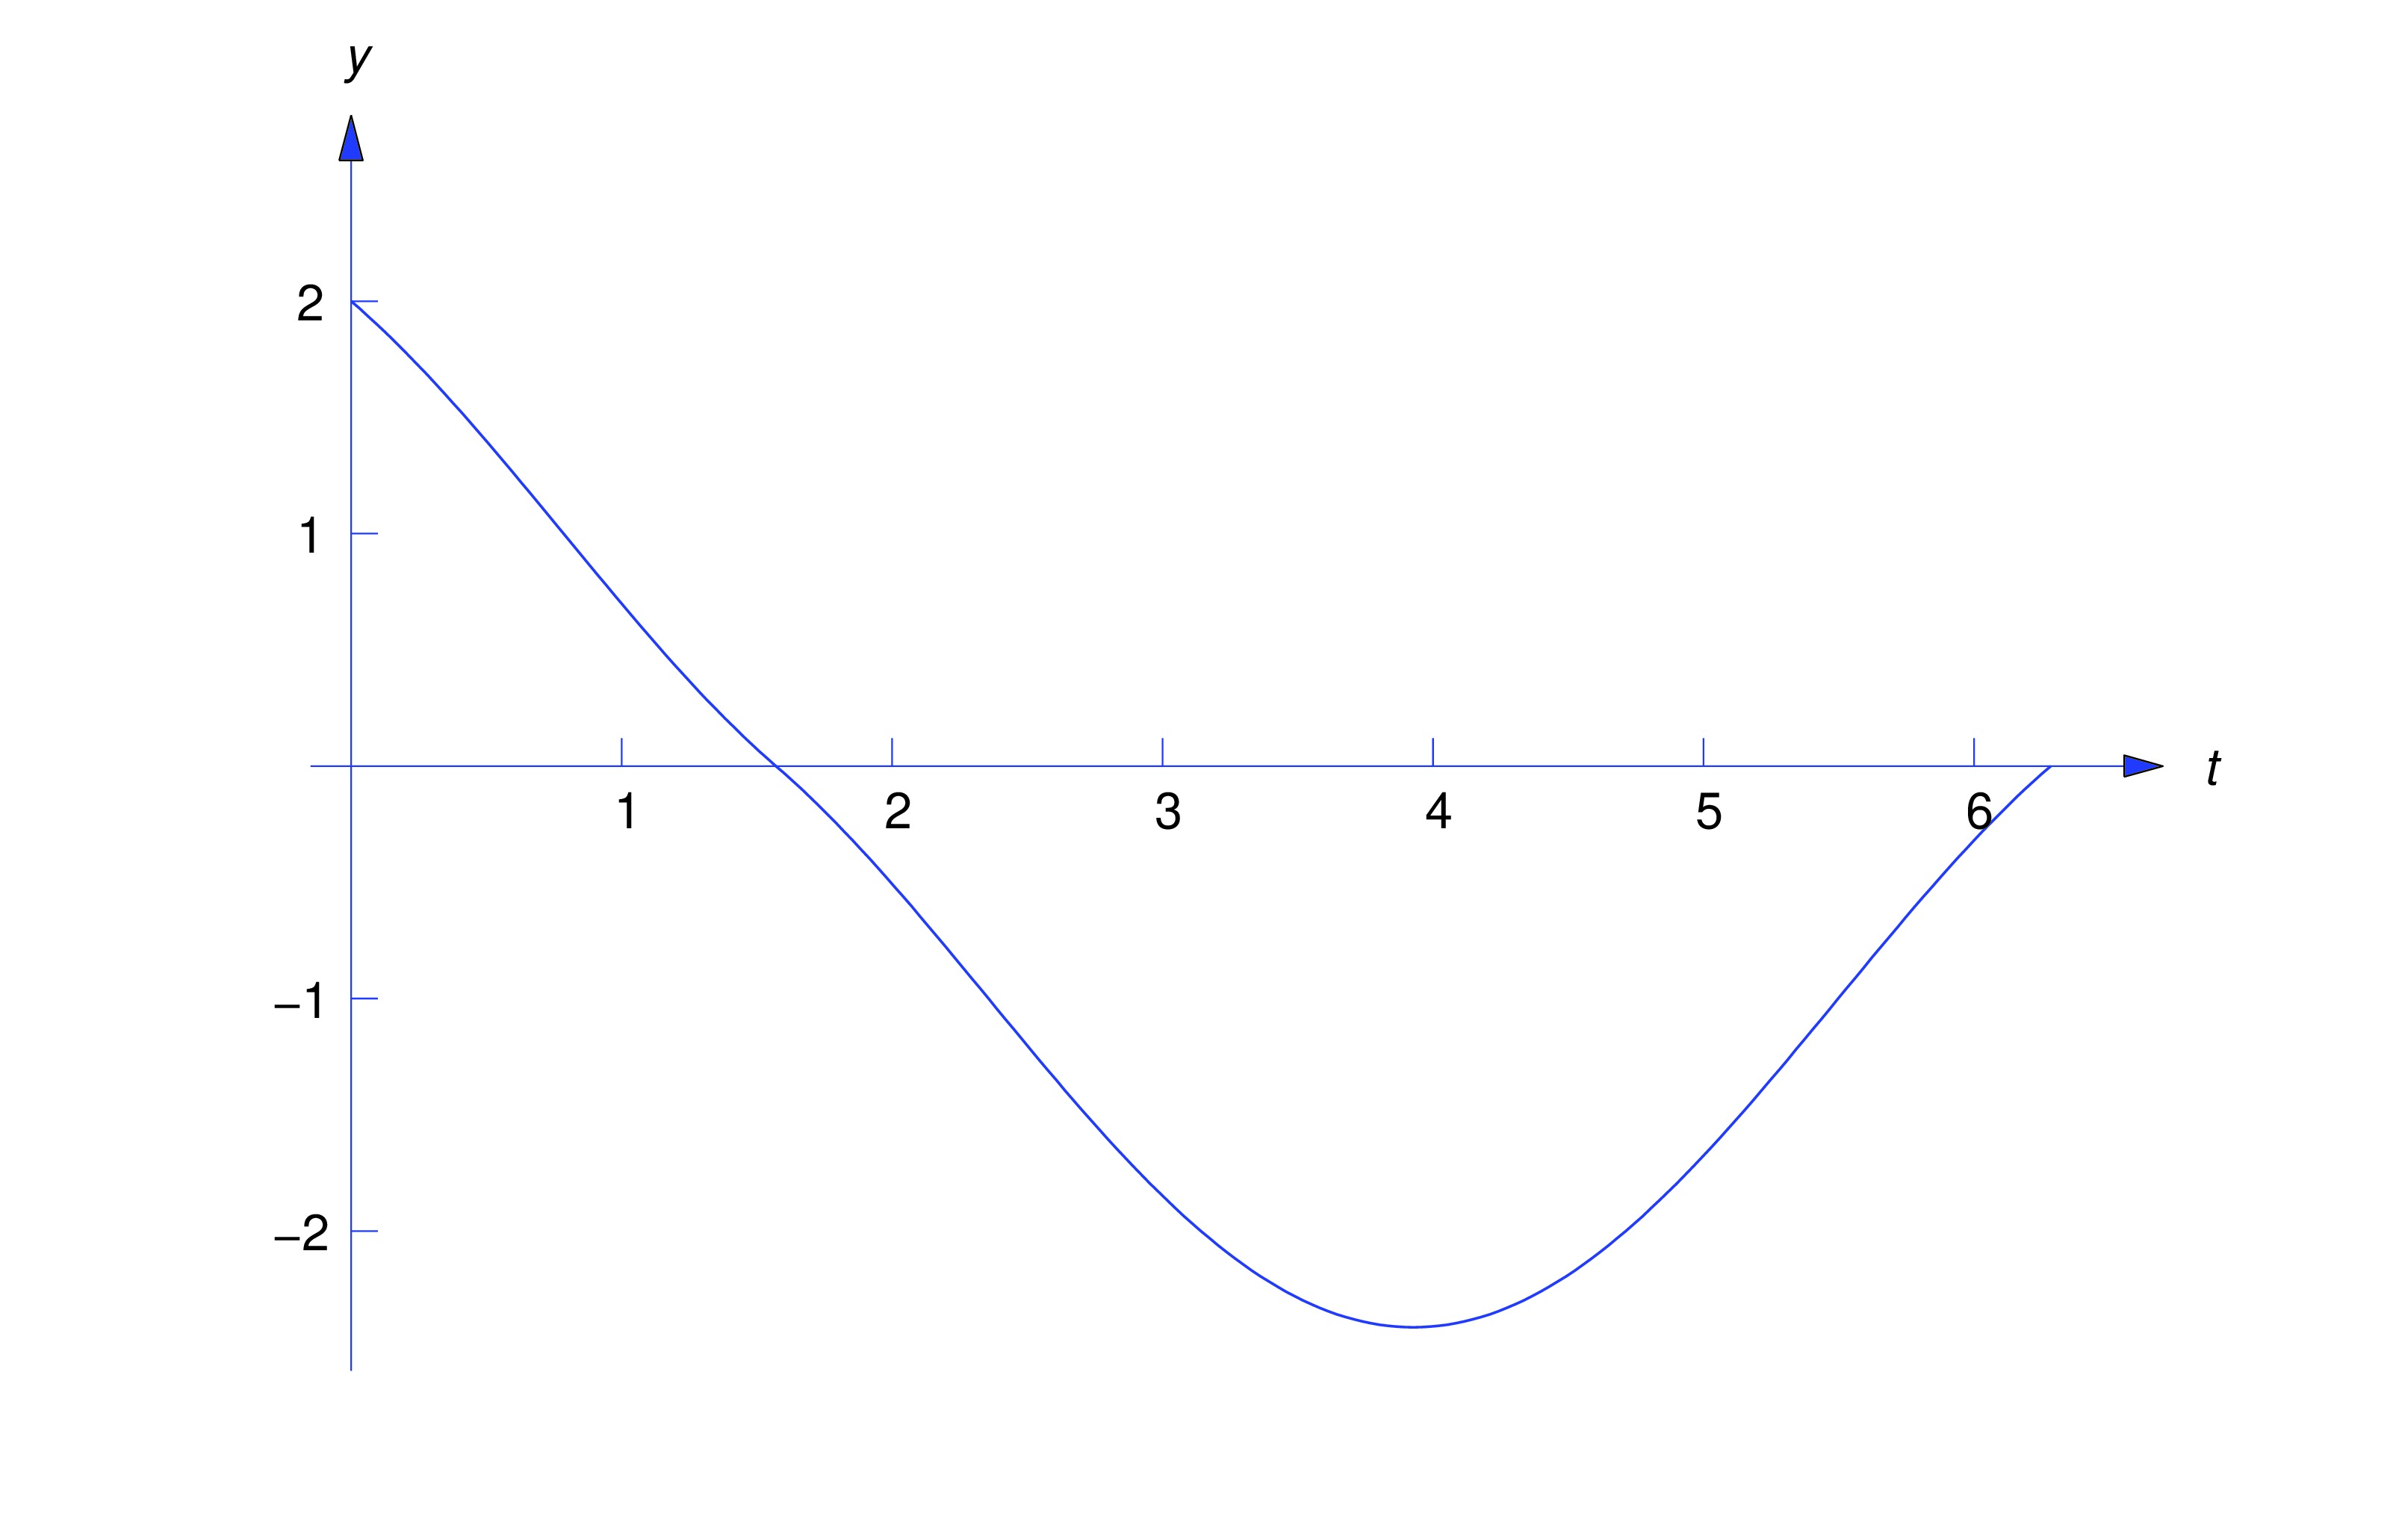
\includegraphics[height=1.5in]{fig080501.jpg}
\end{image}

\end{explanation}
\end{example}

If $f_0$ and $f_1$ are defined on $[0,\infty)$, we can rewrite
\eqref{eq:8.5.2} as
$$
ay''+by'+cy=f_0(t)+u(t-t_1)\left(f_1(t)-f_0(t)\right), \quad  y(0)=k_0,\quad y'(0)=k_1,
$$
and apply the method of Laplace transforms. We'll now solve
the problem considered in Example~\ref{example:8.5.1} by this method.

\begin{example}\label{example:8.5.2}
\space Use the Laplace transform to solve the initial value problem
\begin{equation}\label{eq:8.5.5}
y''+y=f(t), \quad   y(0)=2,  y'(0)=-1,
\end{equation}
where
$$
f(t)=\left\{\begin{array}{cl}
1,&0\leq t<\frac{\pi}{2},\\
-1,&t\geq\frac{\pi}{2}.
\end{array}\right.
$$

\begin{explanation} Here
$$
f(t)=1-2u\left(t-\frac{\pi}{2}\right),
$$
so Theorem~\ref{thmtype:8.4.1} (with $g(t)=1$) implies that
$$
{\cal L}(f)=\frac{1-2e^{-{\pi s/2}}}{s}.
$$
Therefore, transforming  \eqref{eq:8.5.5} yields
$$
(s^2+1)Y(s)=\frac{1-2e^{-{\pi s/ 2}}}{s}-1+2s,
$$
 so
\begin{equation}\label{eq:8.5.6}
Y(s)=(1-2e^{-{\pi s/ 2}}) G(s)+\frac{2s-1}{s^2+1},
\end{equation}
with
$$
G(s)=\frac{1}{s(s^2+1)}.
$$
The form for the partial fraction expansion of $G$ is
\begin{equation}\label{eq:8.5.7}
\frac{1}{s(s^2+1)}=\frac{A}{s}+\frac{Bs+C}{s^2+1}.
\end{equation}
Multiplying through by $s(s^2+1)$ yields
$$
A(s^2+1)+(Bs+C)s=1,
$$
or
$$
(A+B)s^2+Cs+A=1.
$$
Equating coefficients of like powers of $s$ on the two sides of this
equation shows that $A=1$, $B=-A=-1$ and $C=0$. Hence, from
\eqref{eq:8.5.7},
$$
G(s)=\frac{1}{s}-\frac{s}{s^2+1}.
$$
Therefore
$$
g(t)=1-\cos t.
$$
From this, \eqref{eq:8.5.6}, and
Theorem~\ref{thmtype:8.4.2},
$$
y=1-\cos t-2u\left(t-\frac{\pi}{2}\right)\left(1-\cos\left(t-\frac{\pi}{2}\right)\right)+2\cos t-\sin t.
$$
Simplifying this (recalling that $\cos (t-\pi/2)=\sin t)$ yields
$$
y=1+\cos t-\sin t-2u\left(t-\frac{\pi}{2}\right)(1-\sin t),
$$
or
$$
y=\left\{\begin{array}{cl}
1+\cos t-\sin t,&0\leq t<\frac{\pi}{2},\\
-1+\cos t+\sin t,&t\geq \frac{\pi}{2},
\end{array}\right.
$$
which is the result obtained in Example~\ref{example:8.5.1}.
\end{explanation}
\end{example}

\begin{remark}
It isn't obvious that using the Laplace transform to solve
\eqref{eq:8.5.2} as we did in Example~\ref{example:8.5.2} yields a function
$y$ with the properties stated in Theorem~\ref{thmtype:8.5.1}; that is,
such that $y$ and $y'$ are continuous on $[0,\infty)$ and $y''$ has
limits from the right and left at $t_1$. However, this is true if  $f_0$ and $f_1$ are continuous and of exponential order on $[0,\infty)$. 
% A proof  is sketched in Exercises~8.6.~\hspace*{-3pt}\ref{exer:8.6.11}--8.6.\hspace*{-3pt}\ref{exer:8.6.13}.
\end{remark}

\begin{example}\label{example:8.5.3}
Solve the initial value problem
\begin{equation}\label{eq:8.5.8}
y''-y=f(t), \quad   y(0)=-1,  y'(0)=2,
\end{equation}
where
$$
f(t)=\left\{\begin{array}{cl}
t,&0\leq t<1,\\
1,&t\geq 1.
\end{array}\right.
$$
\begin{explanation}
Here
$$
f(t)=t-u(t-1)(t-1),
$$
so, using Theorem \ref{thmtype:8.4.1},
\begin{eqnarray*}
{\cal L}(f)&=&{\cal L}(t)-{\cal L}\left(u(t-1)(t-1)\right)\\
&=&{\cal L}(t)-e^{-s}{\cal L}(t)\\
&=&\frac{1}{s^2}-\frac{e^{-s}}{s^2}.
\end{eqnarray*}
Since transforming  \eqref{eq:8.5.8} yields
$$
(s^2-1) Y(s)={\cal L}(f)+2-s,
$$
we see that
\begin{equation}\label{eq:8.5.9}
Y(s)=(1-e^{-s})H(s)+\frac{2-s}{s^2-1},
\end{equation}
where
$$
H(s)=\frac{1}{s^2(s^2-1)}=\frac{1}{s^2-1}-\frac{1}{s^2};
$$
 therefore
\begin{equation}\label{eq:8.5.10}
h(t)=\sinh t-t.
\end{equation}
Since
$$
{\cal L}^{-1}\left(\frac{2-s}{s^2-1}\right)=2\sinh t-\cosh t,
$$
we conclude from  \eqref{eq:8.5.9},  \eqref{eq:8.5.10}, and
Theorem~\ref{thmtype:8.4.1} that
$$
y=\sinh t-t-u(t-1)\left(\sinh (t-1)-t+1\right)+2\sinh t-
\cosh t,
$$
or
\begin{equation}\label{eq:8.5.11}
y=3\sinh t-\cosh t-t-u(t-1)\left(\sinh (t-1)-t+1\right)
\end{equation}
We leave it to you to verify that $y$  and $y'$ are continuous and
$y''$ has limits from the right and left at
$t_1=1$.
\end{explanation}
\end{example}

\begin{example}\label{example:8.5.4}
 Solve the initial value problem
\begin{equation}\label{eq:8.5.12}
y''+y=f(t), \quad   y(0)=0,  y'(0)=0,
\end{equation}
where
$$
f(t)=\left\{\begin{array}{cl}
 0,&0\leq t<\frac{\pi}{4},\\
\cos2t,&\frac{\pi}{4}\leq t<\pi,\\
 0,&t\geq\pi.
\end{array}\right.
$$
\begin{explanation}
Here
$$
f(t)=u(t-\pi/4)\cos2t-u(t-\pi)\cos2t,
$$
so
\begin{eqnarray*}
{\cal L}(f)&=&{\cal L}\left(u(t-\pi/4)\cos2t\right)-{\cal L}\left(u(t-\pi)\cos2t\right)\\
&=&e^{-{\pi s/4}}{\cal L}\left(\cos2(t+\pi/4)\right)-e^{-\pi s}{\cal L}\left(\cos2(t+\pi)\right)\\
&=&-e^{-{\pi s/4}}{\cal L}(\sin2t)-e^{-\pi s}
{\cal L}(\cos2t)\\
&=&-\frac{2e^{-{\pi s/ 4}}}{s^2+4}-\frac{se^{-\pi s}}{s^2+4}.
\end{eqnarray*}
Since transforming \eqref{eq:8.5.12} yields
$$
(s^2+1)Y(s)={\cal L}(f),
$$
we see that
\begin{equation}\label{eq:8.5.13}
Y(s)=e^{-{\pi s/ 4}} H_1(s)+e^{-\pi s} H_2(s),
\end{equation}
where
\begin{equation}\label{eq:8.5.14}
H_1(s)=-\frac{2}{(s^2+1)(s^2+4)}\quad\mbox{and}\quad H_2(s)=-\frac{s}{(s^2+1)(s^2+4)}.
\end{equation}
To simplify the required partial fraction expansions, we first write
$$
\frac{1}{(x+1)(x+4)}=\frac{1}{3}\left[\frac{1}{x+1}-\frac{1}{x+4}\right].
$$
Setting $x=s^2$ and substituting the result in  \eqref{eq:8.5.14} yields
$$
H_1(s)=-\frac{2}{3}\left[\frac{1}{s^2+1}-\frac{1}{s^2+4}\right]
\quad\mbox{and}\quad
H_2(s)=-\frac{1}{3}\left[\frac{s}{s^2+1}-\frac{s}{s^2+4}\right].
$$
The inverse transforms are
$$
h_1(t)=-\frac{2}{3}\sin t+\frac{1}{3}\sin2t
\quad\mbox{and}
h_2(t)=-\frac{1}{3}\cos t+\frac{1}{3}\cos2t.
$$
From  \eqref{eq:8.5.13} and Theorem~8.4.2,
\begin{equation}\label{eq:8.5.15}
y=u\left(t-\frac{\pi}{4}\right) h_1\left(t-\frac{\pi}{4}\right)+
u(t-\pi) h_2(t-\pi).
\end{equation}
Since
\begin{eqnarray*}
h_1\left(t-\frac{\pi}{4}\right)&=&-\frac{2}{3}\sin\left(t-\frac{\pi}{4}\right)+\frac{1}{3}\sin2\left(t-\frac{\pi}{4}\right)\\
&=&-\frac{\sqrt{2}}{3} (\sin t-\cos t)-\frac{1}{3}\cos2t
\end{eqnarray*}
and
\begin{eqnarray*}
h_2(t-\pi)&=&-\frac{1}{3}\cos (t-\pi)+\frac{1}{3}\cos2(t-\pi)\\
&=&\frac{1}{3}\cos t+\frac{1}{3}\cos2t,
\end{eqnarray*}
 \eqref{eq:8.5.15} can be rewritten as
$$
y=-\frac{1}{3}u\left(t-\frac{\pi}{4}\right)\left(\sqrt{2}(\sin
t-\cos t)+\cos2t\right)
+ \frac{1}{3} u(t-\pi) (\cos t+\cos2t)
$$
or
\begin{equation}\label{eq:8.5.16}
y=\left\{\begin{array}{cl}
0,&0\leq t<\frac{\pi}{4},\\
-\frac{\sqrt{2}}{3}(\sin t-\cos t)-\frac{1}{3}\cos2t,&\frac{\pi}{4}\leq t<\pi,\\
-\frac{\sqrt{2}}{3}\sin t+\frac{1+\sqrt{2}}{3}\cos t ,&t\geq\pi.
\end{array}\right.
\end{equation}
We leave it to you to verify that $y$ and $y'$ are continuous and
$y''$ has limits from the right and left at $t_1=\pi/4$ and $t_2=\pi$
(see figure below).

\begin{image}
 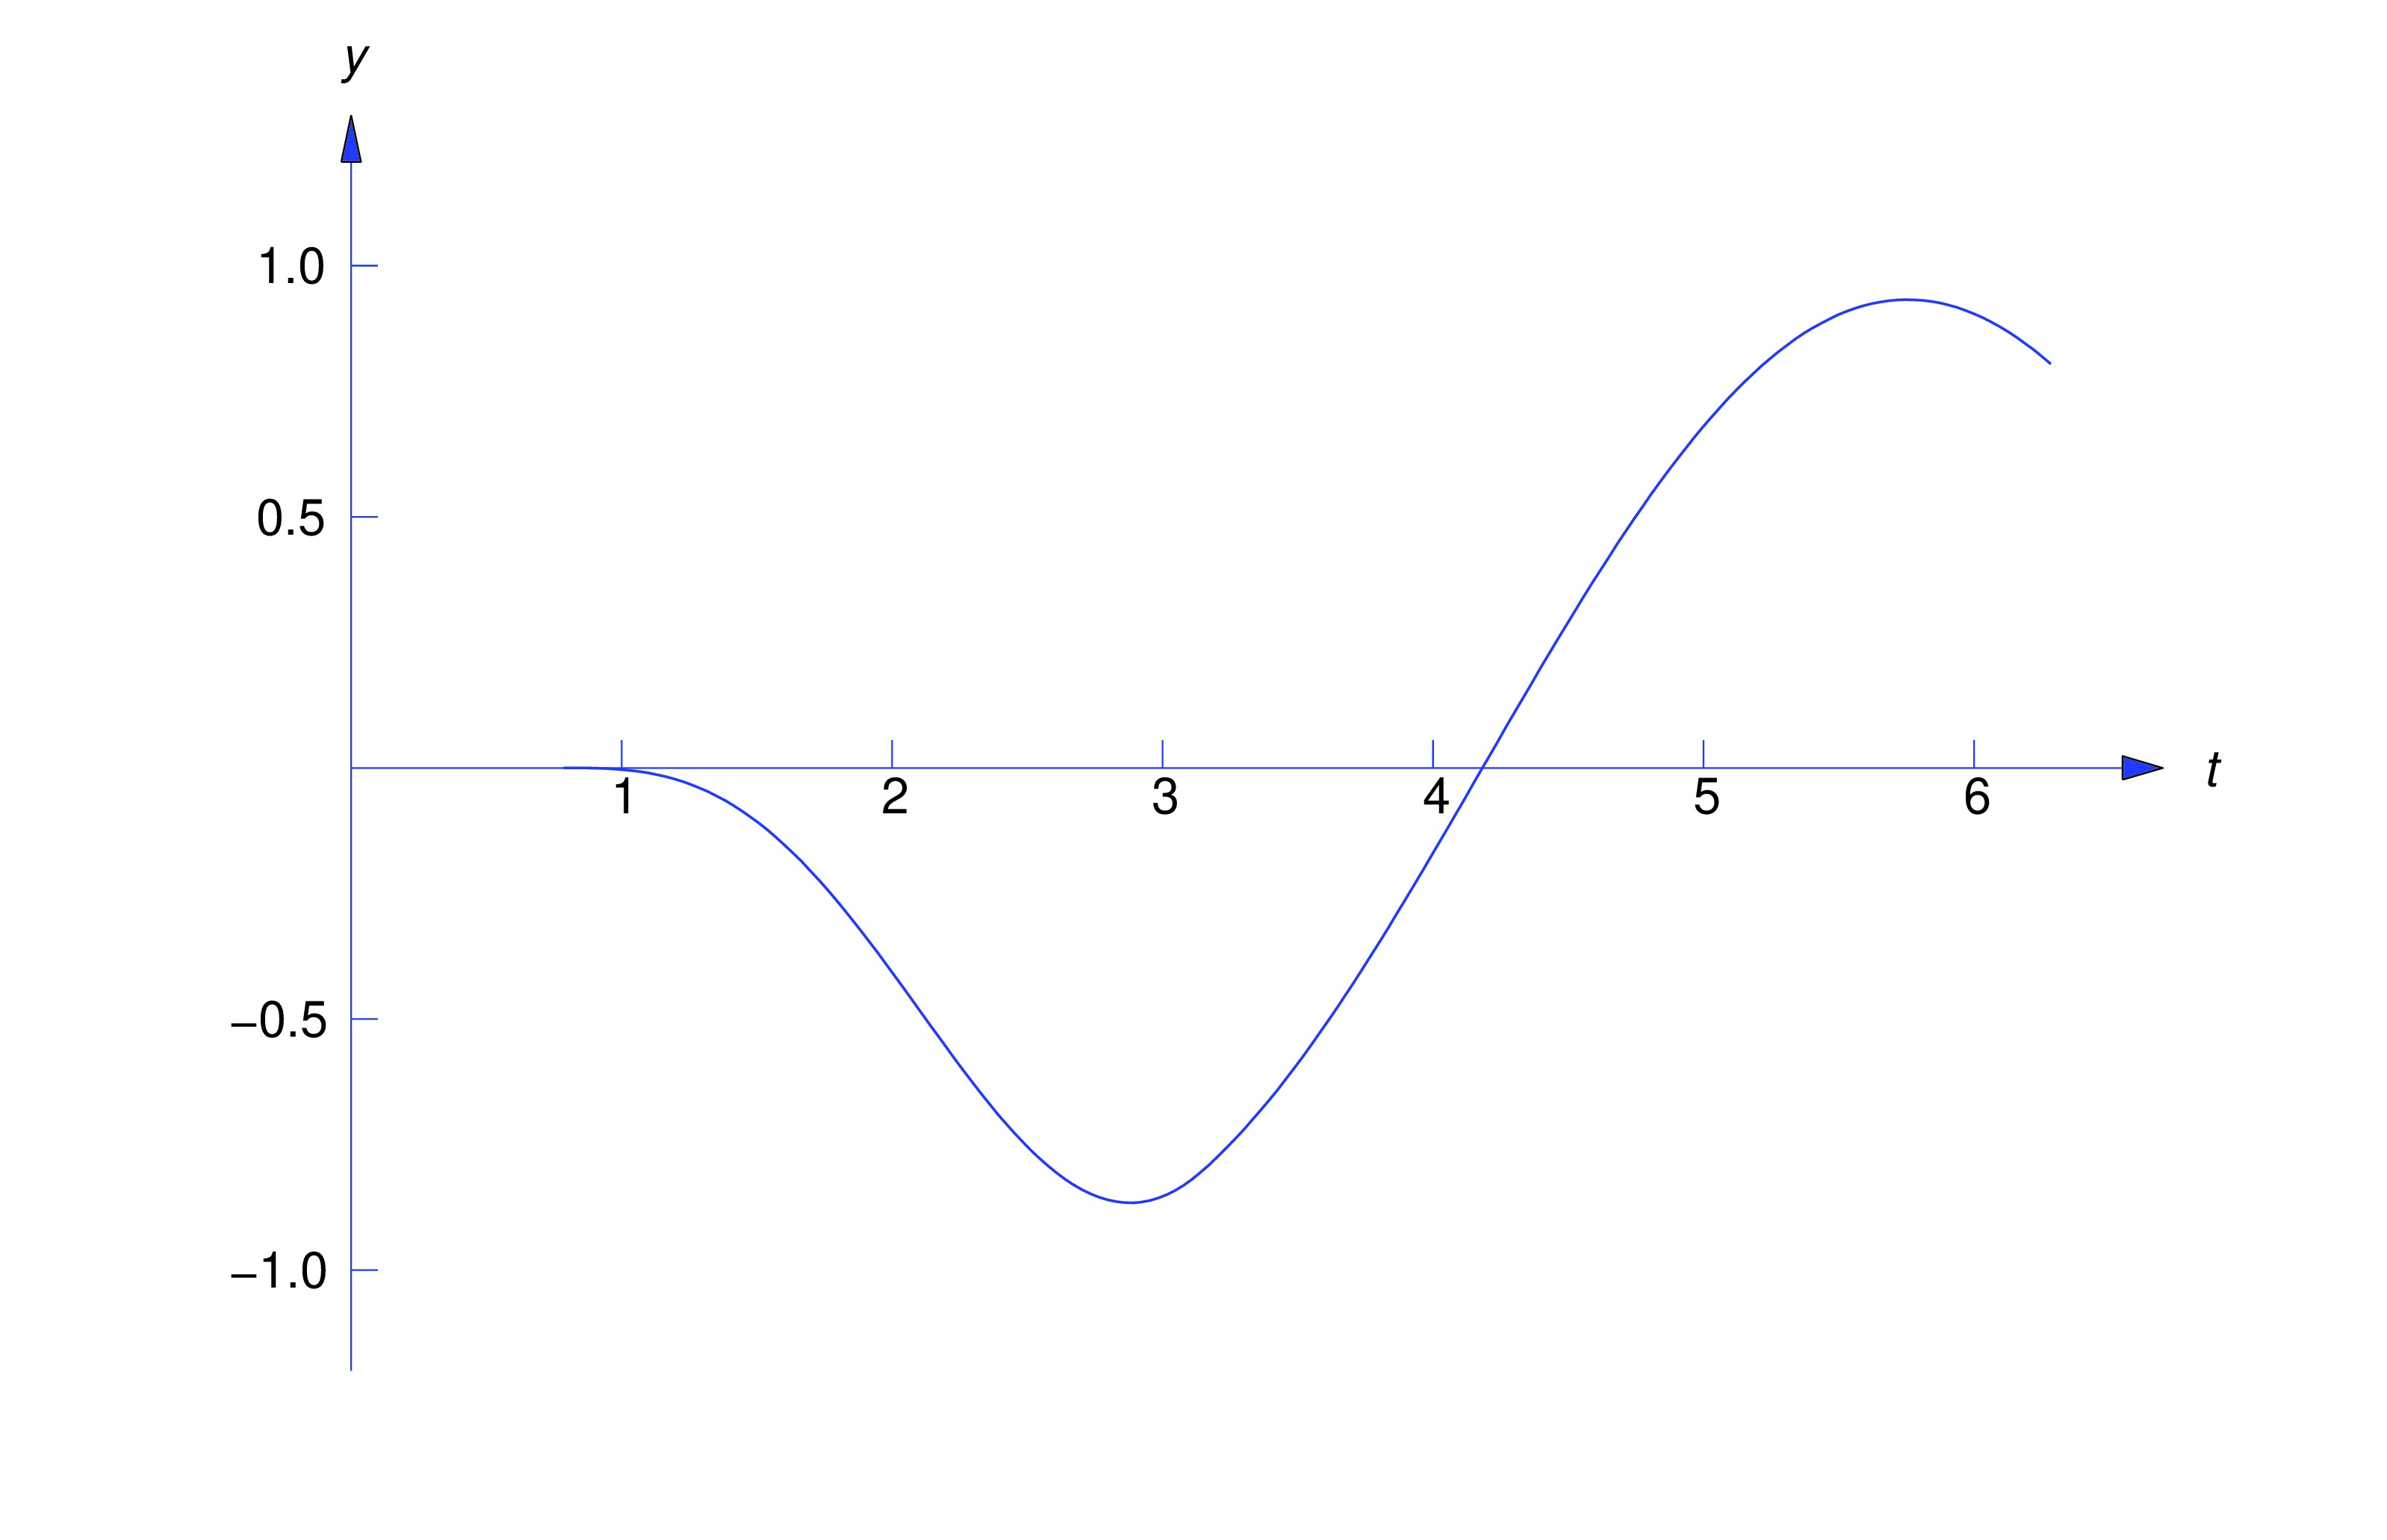
\includegraphics[height=1.5in]{fig080502.jpg}
\end{image}

\end{explanation}
\end{example}

\section*{Text Source}
Trench, William F., "Elementary Differential Equations" (2013). Faculty Authored and Edited Books \& CDs. 8. (CC-BY-NC-SA)

\href{https://digitalcommons.trinity.edu/mono/8/}{https://digitalcommons.trinity.edu/mono/8/}


\end{document}